\begin{savequote}
	Celebrate the fact that you are no longer bound to trivial human conceptions, you are free
\qauthor{Klaus Mikaelson}
\end{savequote}

\chapter{La independencia}
\section{Como alcanzar la independencia}
Si has llegado hasta este punto probablemente te estes planteando esta cuestion. Y es que es cierto que no es algo trivial, yo \textbf{nunca te dare \textit{la solucion}, si no herramientas que considero te ayudaran a construir tu propia solucion}.\\

Esto para mi es una clave de la vida y no es que me desvie del tema, por que la \textbf{proactividad es un punto clave} si queremos ser independientes, si nos ponemos como meta la independencia tenemos que tener claro que tendremos que hacer mucho mucho trabajo que a lo mejor no es reconocido instantaneamente, pero ten por seguro que si has trabajado duro de forma honesta acorde a tus valores, los beneficios vendran por si solos.\\

Esto esta bien, es lo que hace la mayoria de la gente, mirar a hoy, al dia despues, a dentro de un rato, a una semana, a un mes...otro punto clave de la independencia considero que es \textbf{tener una vision de futuro clara} o al menos un camino, como comentaba en otro capitulo no lo tienes que tener todo clarisimo y fijo, pero si que conviene que definas tu camino al menos. Esta vision es lo que te va a ayudar a empujarte hacia ella y a hacer trabajo sin recompensas inmediatas, pues sabes que estas trabajando duro por algo mas alla de lo tangible, por un sentimiento, por una meta. Y diras, pero eso no me va a pagar las facturas, y yo te puedo decir que seguro que si lo hara, aunque te veas en la situacion de tener pocas posesiones materiales o problemas con el dinero, analizalo, pero si de verdad crees en tu vision, el dia llegara en que seras recompensado. Cuantas personas famososas incluso de la lista forbes no perdieron todo antes de llegar a donde estan o empezaron sin nada. Quiero hacer un pequeno apunte y es que cuando digo que definamos nuestro camino esto no es algo estatico, lo bonito de hecho es que mientras que lo vayamos recorriendo, probablemente lo iremos modificando poco a poco.\\

Intentare reflejar este conocimiento teorico con algunas anecdotas que relato a continuacion: En mi universidad un dia estaba hablando con una persona, me dijo que nunca podria llegar alto dentro de una empresa y mucho menos por mi mismo si no era por enchufe. Me parecio bastante curioso y se me quedo marcado, aunque yo creo que elijo mi propio destino y que puedo llegar a donde me proponga pero bueno. El caso es que en uno de los podcast de Fearless Motivation estaban comentando como gente que nace pobre se puede volver rica en terminos economicos por ejemplo, pero tambien en otros terminos como sociales, intelectuales...pero la parte importante venia cuando decian \textit{los padres ricos que nacieron en familias humildes les dan a sus hijos todo, todo menos las condiciones que les llevaron a ellos a ser ricos} a mi forma de ver con esto quieren decir que estos padres cuando eran ninos o adolescentes, sintieron una necesidad de trabajar mas, decidieron perseguir sus suenos y encontraron la manera, que ademas suele ser mas ingeniosa y sufrida en estos casos, de hacerlo sin el apoyo inmediato de sus familiares por que no tenian la capacidad economica para arrancar su empresa por ejemplo. Asi, ante la falta de algo como es el dinero, y el planteamiento de una meta o un sueno, consiguieron ese dinero, y ahora con el pagan todos los suenos de sus hijos que no se veran motivados a encontrar otra manera o trabajar duro por que con pedir el dinero a los padres lo pueden tener todo **(en algunos casos, notese que yo no tengo nada en contra de los padres ricos que se permiten lujos, es solo para exagerar el ejemplo).\\

Esta historia me parece paradojica pero curiosa, a parte me veo en la obligacion moral de comentar el techo que te estas poniendo a ti mismo si te levantas cada manana pensando que no puedes llegar mas alto que x posicion o no puedes llegar a tener mas de x dinero por el mero sitio en el que naciste. Es muy peligroso este sentimiento pero muy facil acoplarse a el pues asi puedes culpar a algo como el sistema de todas tus penurias (te justificas) lo cual es infinitamente mas sencillo que plantarte de cara al mundo y decir yo lo voy a conseguir, voy a trabajar duro y voy a hacer todo lo que este en mi mano por conseguir este sueno, voy a hacer sacrificios, no ire de fiesta, vivire con una politica economica de auesteridad y ahorro, no voy a caer en el consumismo o en otras trampas que me envuelven en una espiral de negatividad, voy a ser verdaderamente responsable y consecuente con mis acciones, si fracaso lo aceptare, aprendere la leccion y comenzare de nuevo pues ahora soy mas sabio y estoy un paso mas cerca de conseguir lo que me he propuesto, nada ni nadie tiene la fuerza psicologica para pararme los pies.



\section{Independencia en la toma de decisiones}
Ahora hablare de otro punto que considero fundamental, como te digo, todo esto son pequenas ideas para que mejores o evalues tu \textit{mindset}. \textbf{Tu eres el unico que toma tus decisiones}, si sientes que es la sociedad en general o un grupo de gente quien toma las decisiones por ti, probablemente estes dentro de una relacion de dependencia. Con esto no te digo que te vuelvas radical de la noche a la manana y digas que te vas a vivir solo, que te vas del trabajo, etc...\textit{(aunque esto puede puede llegar a ser algo positivo en algunos casos, no querria que se entendiera esa idea y no es un consejo que daria a alguien menos si no le conozco)}, lo que te digo es que evalues y que seas consciente de que aunque tu creas que haya cosas que tienes que hacer si o si por que otros te lo han dicho o "por que si", por que asi he nacido, por prejuicios sociales, etc...En ultima instancia tenemos que reconocer que los que tomamos las decisiones somos cada uno de nosotros, aunque esas decisiones sean seguir al rebano. \\

En este ambito, nos tenemos que hacer fuertes, tenemos que comenzar a evaluar las areas en las que estamos siendo dependientes y comenzar a darnos cuenta de que las decisiones que tomamos no estan fundamentadas en ningun criterio que hayamos desarrollado nosotros. Hay que evaluar cada una de estas areas e ir haciendo cambios poco a poco, atreverte a decir no, a preguntar lo que nadie se atreve a preguntar, a cuestionar a los demas siempre con respeto, a plantear ideas que parezcan muy locas y que todo el mundo nos llame locos, que digan que no podemos conseguirlo. Con esto te animo a experimentar diferentes alternativas que te ayuden a recorrer tu camino, ver cual se adapta mejor, pero por favor, se consciente de que \textbf{tu has llegado hasta el sitio donde estas en la vida por tus propias decisiones, y si lo decides puedes cambiar las decisiones que vas a tomar y por tanto cambiar de sitio en la vida}, esto es lo que me parece fundamental, que nada ni nadie te pare.\\

Algo que me parece bastante curioso y me parece una de los efectos mas fascinantes de la vida es como tomamos decisiones en el momento presente, y que luego al evaluarlas desde un momento futuro nos damos cuenta de que podriamos haber tomado otras decisiones mejores. Esto me parece magia, pero a la vez fundamental, y es que repasar algunos eventos en los que tuvimos que decidirnos entre varias alternativas yo lo veo una cosa muy positiva pues podemos ver en el momento presente los diferentes escenarios en los que estariamos si nos hubieramos decantado por otra opcion. Esto es lo que creo que da \textbf{experiencia real} en la vida, ya que al darnos cuenta de que podriamos haber tomado alguna otra decision mejor y alguna otra decision peor, podemos ajustar los parametros para que la proxima vez que nos encontremos ante una situacion con caracteristicas similares, podamos testear la hipotesis que formamos la anterior vez y ver si se materializa.\\
\section{Independencia social}
Este es uno de los temas delicados si tenemos en cuenta los tiempos que corren, especialmente a la hora de escribir esto. A lo mejor soy solo yo el que piensa que la sociedad es generalmente dependiente unos de otros tanto a nivel de paises, organismos e individuos, pero creo que aunque eso fuera cierto, presentar esta idea puede ser interesante, sobre todo teniendo en cuenta que esto no va a ser una mera critica social si no que voy a presentar las alternativas en las que yo creo.\\

Para ilustrar este tema, voy a comentar el caso de un amigo que me mando un video, este consistia de un experimento muy famoso \cite{asch1951effects} que consistia en pocas de palabras de ver la influencia que un grupo podia tener sobre un individuo a la hora de percibir la realidad. Habia varias lineas dibujadas en un papel, y varias personas tenian que decir cual era la mas corta. Lo que no se decia, era que todos los participantes eran actores menos uno. Las primeras veces se veia como la persona "real" decia lo que el pensaba por si mismo, es decir, actuaba de forma independiente, sin embargo, a medida que iban avanzando las rondas, iba dudando mas y mas y terminaba por decir lo mismo que los demas, pensando que su juicio era incorrecto al comienzo, y que sus propios ojos le enganaban a la hora de medir las lineas.\\


Esto me parece extremadamente curioso pues algo que es cuantificable y verificable matematicamente como es la longitud de una linea, y un algoritmo que seria muy sencillo para un ordenador como es calcular la linea de menor longitud, puede tornarse tan complejo en nuestra cabeza por el hecho de que estamos escuchando diferentes opiniones. No digo que tengamos que ser maquinas y que no nos debamos dejar influir por los demas en ciertos aspectos, solo que en aspectos tan fundamentales como estos debemos tener un minimo metodo cientifico con el que operar para ver si es cierto o no. En cuanto a este experimento, yo se que esta en nuestra naturaleza ser seres sociales que nos vemos en mayor o menor medida influenciados por lo que piensan los demas, pero en un caso real similar, tanto nos costaria sacar una regla y medir ? \\

Entonces en que aspectos nos debemos "dejar influenciar"? \\

Como ya he comentado cuando hablaba de los habitos, creo que es fundamental que a la hora de aprender algo nuevo, nos rodeemos de personas que lo potencien. Ahora bien, lo complejo aqui es elegir de que personas nos fiamos y de quienes no en cuanto a lo que nos van a ensenar, pues es posible que lo que nos digan se nos quede grabado si somos muy virgenes en el tema. Ante esta situacion, yo creo que lo mejor es contrastar opiniones, ver diferentes corrientes, por ejemplo si queremos aprender como funciona una sociedad a nivel economico, podemos tener en cuenta algunas opiniones de alguien que se declare comunista y de alguien que siga la escuela espanola o austriaca, os aseguro que las opiniones seran muy distintas. Asi, podremos 
\section{Independencia financiera}

Yo no soy quien para darte lecciones sobre como o en que tienes que gastar o dejar de gastar tu dinero, sin embargo, te ofrezco dos principios que creo que pueden ser interesantes:

\subsection{Disclaimer}

Los contenidos que vas a leer a continuacion pueden ajustarse muy poco a lo que es la realidad al menos en tiempos de escribir este libro, donde lo que se aplica en todos los estados desarrollados es una especie de keynesianismo \cite{guerrero2001desempleo} Esto que quiere decir en pocas palabras?

\begin{itemize}
	\item Estados grandes con bastante poder sobre el pueblo
	\item {Estados <<del bienestar>> basados en recaudar muchos impuestos de los ciudadanos y usarlos para financiar mecanismos, en ocasiones y especialmente en nuestro pais, deficitarios como la seguridad social.\\

		Como ya decia Huerta de Soto: 
		\begin{displayquote}
			La seguridad social no es ni segura ni social
		\end{displayquote}

		\begin{figure}[H]
			\centering
			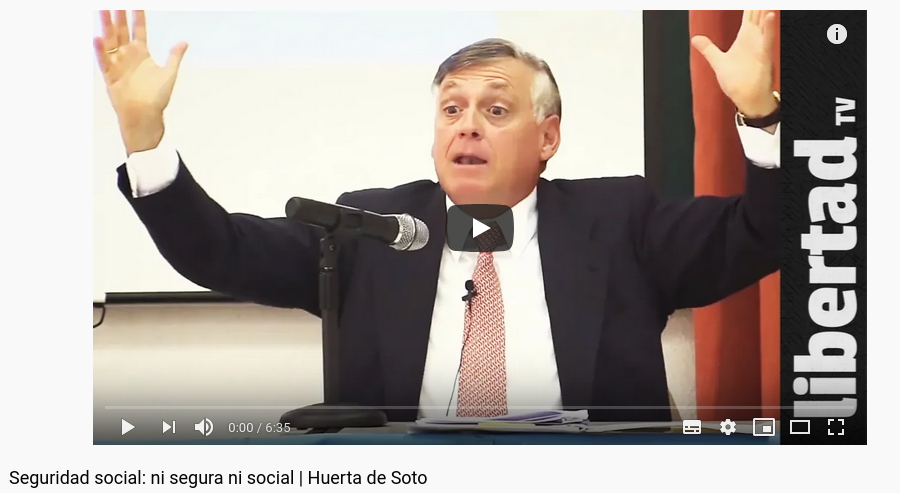
\includegraphics[width=0.75\textwidth]{figures/seguridad_social.png}
			\caption{\href{https://www.youtube.com/watch?v=NWA4nKAQjR4}{video de Huerta de Soto}}
		\end{figure}
		}
	\item{ Los paises se pueden endeudar, parece que infinitamente, por que hay mecanismos para <<imprimir dinero>>  entre ellos destaca el banco central que es <<el diablo de la economia moderna>> 
		\begin{figure}[H]
			\centering
			
\includegraphics[width=0.75\textwidth]{figures/banca_central.png}
			\caption{\href{https://www.youtube.com/watch?v=LNxijjii3eA}{video sobre  la banca central}}
		\end{figure}
		}
\end{itemize}

Mi humilde opinion es que estos principios inducen y animan al descontrol de las cuentas, pero como se puede \textbf{\textit{recibir sin dar nada a cambio}} en cierta medida, pues esto se convierte en un ciclo bastante toxico que algun dia explotara cuando la gente deje de confiar en elsistema y emigre hacia otras soluciones como el \textit{patron oro}  o las \textit{soluciones descentralizadas como el \textbf{bitcoin}\cite{nakamoto2019bitcoin}} \\
		\begin{figure}[H]
			\centering
			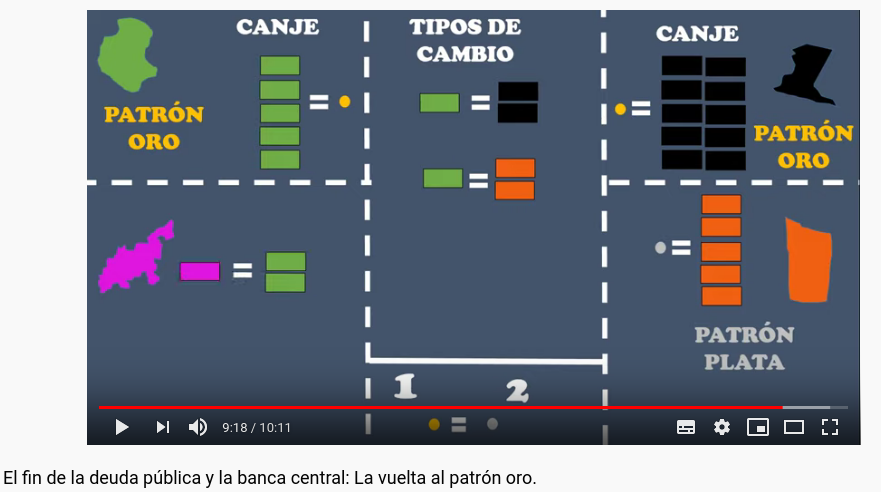
\includegraphics[width=0.75\textwidth]{figures/patron_oro.png}
			\caption{\href{https://www.youtube.com/watch?v=dFA7_wjIq_c}{video sobre el patron oro}}
		\end{figure}

Es por esto, y por que yo con mis pocos anos de vida ya he vivido dos fuertes crisis, la de las hipotecas del 2008 \cite{montalvo2009financiacion} y la de este presente ano, el coronavirus \cite{khafaie2020cross} que yo abogo por una politica economica mas responsable desde el nivel mas bajo y fundamental de la cadena, el individual. A continuacion repaso muy brevemente dos puntos que me parecen fundamentales:

\subsection{Ahorra}

Ahorrar creo que es una de las cosas basicas de cualquier economia, ya estemos hablando a nivel individual, familiar, social o de estado, es basico ahorrar.\\

Por que, te puedes estar preguntando, pues muy sencillo, ahorrar te proporciona la capacidad para adquirir nuevos bienes y servicios. Cuanta mas capacidad de ahorro tengas mas podras comprar, haciendo un ciclo bastante rico propio de una economia prospera, pues si tu consigues dinero que puedes intercambiar por bienes y servicios, quienes los proporcionan tambien obtienen dinero y se va formando esta cadena.\\

\textbf{Haber ahorrado} tambien es fundamental en epocas de crisis como la que estamos viviendo ahora pues aunque quiebre la empresa en la que trabajas o seas despedido y no encuentres la oportunidad de un empleo podrias capear el temporal.\\

Por ultimo pero no menos importante, considero que uno de los mayores beneficios de ahorrar consiste en que cuando tenemos algo de capital y vemos una oportunidad de compra ya sea por ejemplo <<sobre ladrillo>>, en una empresa directamente o en el mercado de valores, podemos atacar sin dudar ni endeudarnos.

\subsection{Invierte}

Cuando hablo de invertir no me refiero unicamente a ir a comprar acciones de empresas en la bolsa de valores. \\

Yo considero una inversion todo lo que obtenemos o perseguimos, sin importar si es o no material, con la intencion de conseguir algun beneficio o rendimiento. Por ejemplo, podrias invertir en una dieta mas saludable o acorde a tus objetivos para acelerar el proceso de alcanzarlos, en este caso estarias comprando comida a cambio de mantener un cierto <<look>> o de alcanzar un fisico estetico o de simplemente estar mas sano. Das algo (dinero para comprar) y recibes algo a cambio (salud y estetica por ejemplo). Otro ejemplo seria comprar un buen ordenador para desarrollar tu trabajo en el caso de ser informatico por ejemplo. Como veremos en un posterior punto, yo no considero que tengas que gastarte una cantidad significativa de dinero para conseguir esto, hacieno un simil con la bolsa de valores seria como comprar acciones de una empresa cuando estan a 5\$, que otra persona las compre cuando estan a 90\$ y que actualmente se encuentren a 100\$. Con esto lo que intento decir es que tanto en la bolsa como al comprar un ordenador y todas las situaciones podemos hacer mejores o peores inversiones, el que se ha gastado solo 50\$ digamos por ejemplo, en un ordenador, pero es capaz de desarrollar el mismo trabajo que el que ha gastado 900\$ por ejemplo, suponiendo que el trabajo que realizan los dos es igual y les reportase 1000\$ de beneficio, habra hecho sin duda una inversion muchisimo mejor, mas inteligente.\\

Pero no nos equivoquemos, yo soy de los que piensa que algunas de las inversiones mas importantes que se hacen no se pagan con dinero, pero sin embargo reportaran enormes beneficios. Con esto me refiero a que la inversion mas importante que podemos hacer no tiene por que ser en nada material si no en nosotros mismos. A lo largo de estas paginas hemos hablado de como la independencia nos puede ayudar y aportar enormes beneficios, pero esto no se contruye con dinero, es un estado mental, un <<mindset>> que no podemos comprar. Asi, quiero decir que no podemos comprar valores. Por ejemplo, si tratasemos de pagar a alguien para que nos ayudase a hacer ejercicio pero nosotros por dentro no tuvieramos ambicion, determinacion, constancia y fuerza, no llegariamos muy lejos. 

Quizas te podrias estar preguntando que tiene todo esto que ver con la independencia, es muy sencillo. A la hora de hacer inversiones es normal en un primer momento tomar como referencia de buena inversion las inversiones que hace la mayoria de la gente, pero estas no tienen por que ser las mejores, esto es por lo que debemos ser independientes a la hora de invertir en lo que sea.\\

Eso si, para ser capaz de anticiparse o de poder sustentar opiniones distintas al resto y por tanto poder realizar inversiones distintas hay que aprender mucho sobre los temas que nos interesan y en la mayoria de las ocasiones esto es un trabajo duro que no veremos recompensado inmediatamente si no cuando realicemos la inversion y conozcamos el resultado sabiendo si lo hemos hecho mejor o peor que el que no se informo sobre el tema.\\

Aunque creo que puedo adelantar sin problema que el que conoce un tema a fondo es capaz de realizar mejores inversiones que los demas, animo a la gente a que prueben esta metodologia antes de lanzarse a comprar un producto, adquirir un servicio o invertir tiempo en una actividad. En mi experiencia es seguro tambien que cuanto mas vayas profundizando, mejores inversiones vas a ir realizando, pues pensar que la primera inversion que realices sera increible es algo que creo que dista de la realidad. Esto es como todo, se aprende haciendo.

\section{Independencia en la informatica}

En esta parte vamos a hablar de que considero yo que es la independencia en informatica y como alcanzarla o perseguirla. Para esto dividire el apartado en dos, constara de una primera parte en la que hablaremos brevemente sobre el hardware, una segunda sobre el software y al final dare una nota.

\subsection{ Hardware }

Cuando hablamos de independencia en el hardware, estoy haciendo referencia a varias caracteristicas que se juntan para ofrecer lo mejor. 

La primera de estas partes es la habilidad que tenemos para saber lo que "gastan", o los recursos que consumen las aplicaciones que utilizamos, esto es fundamental en un primer momento a la hora de elegir un hardware, pues si las aplicaciones que utilizamos son las de uso comun general, por ejemplo navegadores de internet y aplicaciones de ofimatica, no parece tener mucho sentido ir a por una cpu de gama alta o muy alta. El sistema funcionara a la perfeccion, pero estaremos desperdiciando ese hardware que probablemente "pida" un uso mas intensivo. Es como comprarse un coche de 100.000\$ para llevar a los chicos al colegio...Nos resultara mucho mas costoso que si elegimos un coche normalito que sea fiable incluso de segunda mano por lo que obtendremos una rebaja sustancial, asi podriamos \textbf{ completar la misma tarea con poca diferencia en rendimiento por una fraccion del precio. } De la misma forma, en vez de comprar los componentes mas potentes para nuestro ordenador, sabiendo que probablemente no les vayamos a dar un uso intensivo ni la mitad del tiempo, te recomiendo buscar componentes que ofrezcan menor rendimiento a mucho menor precio, incluso informarte y rebuscar entre componentes algo antiguos, estoy seguro de que te podria llegar a sorprender lo barato que puede resultar un ordenador que haga lo que tu necesites.

Otro aspecto muy importante es la capacidad que tiene el hardware para ser \textbf{ extensible }, esto es, que si comenzamos en el mundo de la informatica con un procesador de gama baja, pongamos un intel core 2 duo por ejemplo, pero pasado un tiempo nos damos cuenta de que necesitamos algo mas potente por que las tareas que realizamos son demasiado pesadas, tener la capacidad de poder cambiar ese componente con facilidad. Esto se hace especialmente dificil en el mundo de los portatiles modernos, que son casi "de usar y tirar" y si quieres uno que te dure mucho lo que tienes que hacer es gastar mas. Yo estoy en contra de esto en la mayoria de los casos, hay marcas que hacen portatiles que son muy faciles de modificar, no hace falta ni si quiera llevarlo a un tecnico. Por ejemplo lenovo con sus thinkpad, especialmente los antiguos incluso los de IBM. En ordenadores de sobremesa es relativamente mas sencillo hacer algun cambio de componentes si elegimos una configuracion inicial interesante y apta para ello. Esto por ejemplo hablando de la cpu se logra eligiendo una placa base cuyo socket soporte diferentes gamas de la misma cpu, por ejemplo un i3, i5 e i7. 

Estoy hablando bastante de las cpus, pero otra caracteristica importante a la hora de plantearnos cambiar algun componente del ordenador o incluso cambiar de ordenador es reconocer que va mal o "lento". Si por ejemplo lo que pasa es que cuando vemos peliculas estas tardan mucho en renderizar o incluso no las podemos ver a la resolucion que quisieramos y ademas todo el sistema es muy lento y encima produce mucho calor o ruido, es decir, si todas las partes del ordenador nos dan problemas es buena idea quizas pensar en cambiar de software y en ultima instancia de ordenador. Por otro lado si lo unico que pasa es que el sistema se siente lento, no debemos pensar de primeras en tirarlo y comprar otro, es buena idea por ejemplo investigar el tipo de disco que tiene, ya que si es uno mecanico puede que esa sea la fuente de los problemas, y es mucho mas barato comprar una unidad de estado solido (SSD) y sustituirlo en el equipo que comprar un equipo nuevo. 

Si no estas teniendo una buena experiencia con tu ordenador o crees que no te esta ofreciendo todo lo que necesitas te recomiendo hacer varias consideraciones como investigar la posibilidad de instalar otro sistema operativo, ya que probablemente tengas windows y esto sea la mayor fuente de problemas. Asi podrias investigar algo como instalar un sistema operativo Linux, o investigar los componentes hardware de tu equipo para ver si logras identificar algun cuello de botella importante y ver si es posible cambiar esa parte.

Como nota final he de decir que a mi personalmente me gusta comprar hardware de segunda mano, considero que es un buen mercado por que hay gente que consume y tira los equipos sin saber muy bien que a lo mejor alguna de las piezas de las que va a deshacerse es de mucha calidad y aunque sea antigua puede durar mucho tiempo mas con un mantenimiento adecuado. Yo me monte un sistema asi, con una placa P6T deluxe V2 que va de lujo y que tiene mucha mucha calidad, la compre a una fraccion del precio de lo que cuesta, compre una cpu intel i7 (era la unica opcion que conocia en el momento, ahora he aprendido que se pueden instalar algunos intel Xeon) 4gb de ram y una unidad de estado solido. Esto y algunas piezas mas que hacen falta me costo menos de 200\$ y es un sistema que lleva ya conmigo 2 anos y que durara bastante mas. En cuanto a portatiles, estoy orgullosos de decir que estoy realizando todo este trabajo desde un IBM/Lenovo Thinkpad T60, un portatil de 2006, que funciona a la perfeccion. Le instale algo mas de memoria ram y una unidad de estado solido y va como un tiro. Se le puede tambien cambiar la cpu lo cual hare e incluso la pantalla...La mejor parte es que me costo 50\$ !

\subsection{ Software }

Cuando me monte mi primer ordenador de segunda mano me di cuenta de que Windows costaba mucho dinero, y aunque podia hacer algun apano para que me costase menos, decidi irme por un sistema linux, Ubuntu, que funcionaba bastante mejor. A medida que me fui adentrando en el mundillo me di cuenta de que se pueden conseguir setups software que usan muy poquitos recursos hardware y desde entonces es una de mis metas conseguir un setup hardware + software que sirva para realizar tareas cotidianas sin comproisos. Algunos ejemplos geniales de esto son los SOC \textbf{INSEERTAR REFERNCIA} como las Raspberry Pi (en concreto la version 4) \textbf{INSERTAR IMAGEN}, que son un dispostivo que ofrecen un ordenador con buen rendimiento, mas del que mucha gente necesita, por menos de 100\$.

Centrandonos ahora en el ambito del software, pronto descubri que algunas aplicaciones graficas, o GUI, son en bastantes casos extremadamente ineficientes, pues lo unico que hacen es poner de forma grafica con botones y menus (esto gasta muchos recursos hardware) lo que es o podria ser realmente una aplicacion de consola con las mismas opciones y menus y consumiendo muchos menos recursos...

Como ejemplo pongamos los IDE, como Eclipse \textbf{INSERTAR REFERENCIA} y eso que este no es el peor ejemplo que se me ocurre pues al menos es de codigo abierto, pero sirve para ejemplificar lo que quiero demostrar. Esta aplicacion nos proporciona un entorno grafico con muchos paneles y botones ( que son muy liosos, no es facil encontrar las opciones... ) todo ello para ser capaces de escribir un texto (codigo) en un panel y poder darle a un boton verde que compila el codigo y lanza la aplicacion que estemos construyendo. En la facultad recuerdo que paso que una clase entera de alumnos suspendio un examen por que el entorno estaba mal configurado, y es que la configuracion de estos entornos puede llegar a ser infernal. Yo opto por tener mas control sobre lo que estoy haciendo y simplificar los procesos, independizando cada uno de los pasos que hay que dar pero consiguiendo mucha mas velocidad y mejor rendimiento... Pongo un ejemplo de como estoy haciendo este poryecto o como hago otros que requieren codigo:

\begin{itemize}

\item Edito un archivo de texto en un editor como vim, pero hay otros e incluso puede ser uno grafico que sea muy ligero, yo usaba gedit antes cuando usaba gnome. 

\item Compilo ese archivo con el compilador que yo quiero y que se que va a funcionar y las opciones o flags que me convienen.

\item Lanzo la aplicacion , lo cual es trivial pues en el paso anterior se me ha generado un ejecuable.

\item Por ultimo repito todos los pasos anteriores hasta que tengo el producto final. Si hay que debugear la cosa se puede poner un poco mas compleja, pero una vez aprendes a usar minimamente gdb y a debugear sobre el codigo en la ejecucion del programa, todo se vuelve mas sencillo.

\end{itemize}

Y algunos direis, vale, esto puede estar bien, pero es mucho mas lento y tengo que hacer mas trabajo que si estoy en un entorno y le doy a un boton. Aqui entra la magia de este software, pues al ser muy extensible puedo configurar de forma sencilla y segura un boton en el teclado por el cual se pasa la ruta del archivo que estoy editando a un script que se llama compilar y que tiene una distincion de casos segun la extension del archivo y ahi especifico los compiladores que quiero segun el caso. Asi:

\begin{itemize}

\item
logro tener mucho control, por que yo elijo cada una de las partes segun mis preferencias
\item fiabilidad, por que los mecanismos usados son practicamente atomicos, hay nula o poca configuracion de por medio
\item velocidad, pues una vez controlo los dos puntos anteriores puedo optimizar el proceso automatizandolo a mi gusto.

\end{itemize}

Esta es la base de como uso yo un ordenador, no me conformo con lo que viene dado en un cierto sistema operativo, como por ejemplo Ubuntu. Me gusta toquetear e instalar como interfaz grafica un Tiling window manager \textbf{INSERTAR REFERENCIA AQUI!} como xmonad o dwm \textbf{INSERTAR REFERNCIA AQUI!} y construir "mi propio sistema operativo", esto es, elegir las aplicaciones que ami me gustan, configurarlas y optimizarlas segun mis necesidades. Asi puedo elegir como editor neovim \textbf{INSERTAR REFERENCIA}, como navegador de internet Lynx \textbf{INSERTAR REFERENCIA} , w3m \textbf{INSERTAR REFERENCIA} , surf \textbf{INSERTAR REFERENCIA} o brave \textbf{INSERTAR REFERENCIA}. Puedo automatizar tareas o construir mis propias aplicaciones como mi navegador de ficheros \textbf{INSERTAR REFERENCIA} sobre otras aplicaciones super extensibles como dmenu \textbf{INSERTAR REFERENCIA}, etc etc...  

Asi, te animo a identificar software en tu sistema que es ineficiente e investigar cuales son las alternativas y si hay alguna que resulte mas interesante. Un ejemplo bueno para el publico general son los editores de PDF, los de adobe o similares pueden resultar en desesperanza por lo que tardan en cargar o lo que pueden llegar a costar, sin embargo hay aplicaciones como Xournalpp que te podrian sorprender.

Por ultimo en este apartado me gustaria hacer una mencion especial a los programas online o en la nube que ofrecen servicios muy interesantes y no requieren de instalar. Mi opinion personal es que no los uses a menos de que seas consciente que es probable que algunos de esos programas esten obteniendo redito economico, vendiendo tu informacion por ejemplo, a cambio de que los uses...Sin embargo esto lo considero buena opcion si la nube que usas es tuya, por ejemplo puedes hacer una instalacion de Nextcloud \textbf{INSERTAR REFERENCIA} que es fantastico para esta tarea, en un servidor fisico en tu casa o uno alquilado en un proveedor como DigialOcean \textbf{INSERTAR REFERENCIA} y asi asegurar lo maximo posible que tu eres el unico "beneficiario" del uso de ese tipo de programas, pero la idea de poder usar programas que serian muy pesados para nuestro dispositivo, alojandolos en servidores mas potentes me parece una idea genial.
